\begin{frame}
\frametitle{Attachmnet Description}
\begin{columns}


\column{.55\textwidth}


\begin{itemize}
\item Abbiamo un solo attachment: una delle immagini della swapchain
\item Vogliamo pulire l'attachment prima di utilizzarlo per la prima volta
\item Volgiamo mantenere il contenuto dell'attachment quando il render pass termina
\item Non ci importa del layout dell'attachment prima di iniziare il render pass
\item Quando il render pass termina, volgiamo passare a un layout che renda ottimale la presentazione dell'attachment
\end{itemize}


\column{.25\textwidth}

\begin{figure}[ht]
    \centering
    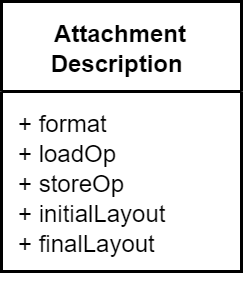
\includegraphics[scale=0.3]{images/SlidesClearWindow/AttachmentDescription.png}
\end{figure}

\end{columns}
\end{frame}
